\documentclass[prez_parietal.tex]{subfiles}
\begin{document}


%---------------------------------------------------------------------------
\subsection{LGCD}
%---------------------------------------------------------------------------

\begin{frame}[t]
\frametitle{Coordinate Descent (CD)}
	
	Minimize
	\[
	Z^{*} = \argmin_{Z}\| X - \sum_{k=1}^K\pmb D_k *  Z_k\|_2^2
			+ \lambda\| Z\|_1
	\]
	Update one coordinate at each iteration.\\[1em]
	\begin{enumerate}
		\item<1-> Select a coordinate $(k_0, t_0)$ to update.
		\item<2-> Compute a new value $Z'_{k_0}[t_0]$ for this coordinate
	\end{enumerate}
	\only<3>{\vskip3em$\Rightarrow$ Converges to the optimal point for CSC problem in $\bO{\frac{1}{q}}$ iterations.}

\only<1>{
	Three algorithms:
	\begin{itemize}\itemindent1em
		\item Cyclic updates; $\bO{1}$  \mycite{Friedman2007}
		\item Random updates; $\bO{1}$ \mycite{Nesterov2010}
		\item Greedy updates; $\bO{KL}$ \mycite{Osher2009}
	\end{itemize}
}
\only<2>{
	For convolutional CD, we can use optimal updates:
	$$
		Z'_{k_0}[t_0] = \frac{1}{\|\pmb D_{k_0}\|_2^2}\text{Sh}(\beta_{k_0}[t_0], \lambda),
	$$
	with {\small $\text{Sh}(y, \lambda) = \text{sign}(y)(|y| - \lambda)_+$}.
	\cite{Kavukcuoglu2013} showed this can be done efficiently, with $\mathcal O(KW)$ operations.
	
	\strongpoint{Local operations}
}
\end{frame}




\begin{frame}{Locally greedy coordinate descent (LGCD) \mycite{Moreau2018}}


We introduced the LGCD method which is an extension of GCD.\\
{
    \centering
    \inputTikZ{.7}{LGCD}
}

\only<1-2>{
    \vskip1em
    GCD has $\mathcal O(K\widetilde{T})$ computational complexity.\\[1em]
    \only<2>{But the update itself has complexity $\mathcal O(KL)$}
}
%
\visible<3->{
    With a partition $\mathcal C_m$ of the signal domain $[1, K]\times [0, \widetilde{T}[$,
    \[
    \mathcal C_m = [1, K]\times [\frac{(m-1)\widetilde{T}}{M}, \frac{m\widetilde{T}}{M}[
    \]%
}%
\visible<4->{%
    The coordinate to update is chosen greedily on a sub-domain $\mathcal C_m$\\[1em]
    
    {\centering$\frac{\widetilde{T}}{M} = 2L-1~~\Rightarrow~~\mathcal O$(Coordinate selection) = $\mathcal O$(Coordinate Update)\\[1em]}
    
    The overall iteration complexity is $\mathcal O(KL)$ instead of $\mathcal O(K\widetilde{T})$.
    \strongpoint{Efficient for sparse $Z$}
}


\end{frame}

\begin{frame}{Fast optimization}
Comparison of the coordinate selection strategy for CD on simulated signals\\
We set $K=10$, $L=150$, $\lambda = 0.1 \lambda_{\max}$\\[1em]
\centering
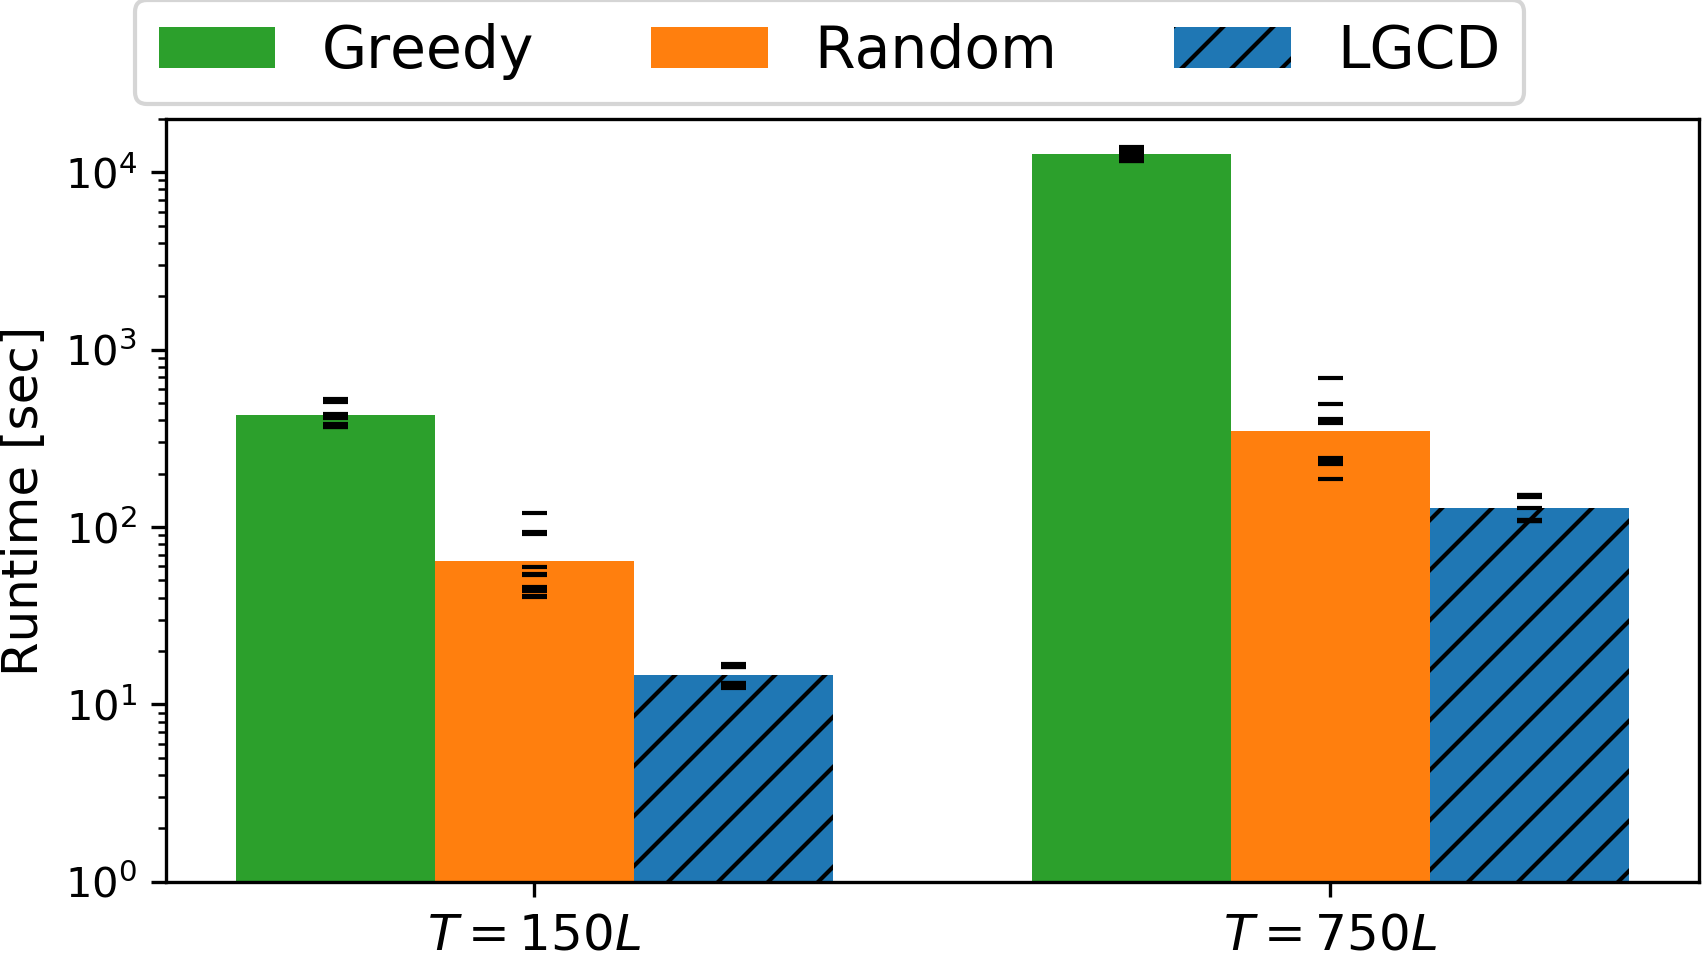
\includegraphics[width=.9\textwidth]{CD_strategies_comparison.png}
\end{frame}




%---------------------------------------------------------------------------
\subsection{DICOD}
%---------------------------------------------------------------------------


\section{Distributed optimization for CSC}

\parttitleframe{Moreau2019,Moreau2018}



%\begin{frame}{Distributed Convolutional Coordinate Descent (DICOD)}
%\vskip1em
%
%$Z$ is the coding signal of length $L$.\\[.5em]
%Each core $\mathcal C_m$ is responsible for the updates of a segment
%$\left \{ m \left\lfloor\frac{L}{M}\right\rfloor , \dots
%(m+1) \left\lfloor\frac{L}{M}\right\rfloor -1 \right \}$ .\\[.5em]
%
%\inputTikZ{.75}{dicod_tikz.tex}
%\end{frame}



\begin{frame}{Weak dependence of the coordinate updates}
The update of the $W$ coordinates $(k_w, \omega_w)_{w=1}^W$ with additive update $\Delta Z_{k_w}[\omega_w]$ changes the cost by:
\begin{align*}
\Delta E =
\overbrace{\sum_{i=1}^W\Delta E_w}^{
    \text{iterative steps}}
- \underbrace{\sum_{w \neq w'}(d_{k_w} * d_{k_{w'}}^\Lsh)[\omega_{w'} - \omega_w]
    \Delta Z_{k_w}[\omega_w] \Delta Z_{k_{w'}}[\omega_{w'}]}_{
    % \Delta Z_{k_w}[w] \Delta Z_{k_{w'}}[w']}_{
    \text{interference}}, \label{eq:interf}
\end{align*}

\strongpoint{If the updates are far enough, they can be considered as independent.}
\end{frame}

\begin{frame}{Distributed Convolutional Coordinate Descent (DICOD)}

{
\centering
\inputTikZ{.7}{DICOD}\\
}
\vskip1em
\begin{itemize}[<+->]\itemsep1em
\item Split the coordinates in continuous sub-segment
$\mathcal S_w = \left[\frac{(w-1)T}{W}, \frac{wT}{W}\right[$.
\item Use CD updates in parallel in each sub-segment.
\item Notify neighbor workers when the update is on the border of $\mathcal S_w$.
\item What do we do when two updates are interfering?
\end{itemize}

\end{frame}



\begin{frame}{DICOD convergence \mycite{Moreau2018}}
\setbeamercolor{my title}{bg=primary!60, fg=secondary}
\setbeamercolor{my body}{bg=white, fg=black}

DICOD converges to the solution of the CSC for 1D signals without having a control mechanism on the interference.\\[1em]

\begin{beamerboxesrounded}[upper=my title,lower=my body,shadow=true]{
        \usebeamerfont{block title}Theorem (Convergence of DICOD)}
    We consider the following assumptions:\\[.3em]
    {\bf H1: }
    If the cross correlation between atoms of $\pmb D$ is strictly smaller than 1.\\[.3em]
    {\bf H2: }
    No cores stop before all its coefficients are optimal.\\[.3em]
    {\bf H3: }
    If the delay in communication between the processes is inferior to the update time.\\[1em]
    Under these assumptions, the DICOD algorithm converges asymptotically to the
    optimal solution $Z^*$ of CSC.
\end{beamerboxesrounded}

\end{frame}


\begin{frame}
\definecolor{fista}{RGB}{192,192,0}
\definecolor{rcd}{RGB}{0,128,0}
\definecolor{cd}{RGB}{255, 0, 0}
\definecolor{dicod}{RGB}{0,0,255}

\frametitle{Numerical Experiments}
Test on long signals generated with Bernoulli-Gaussian
coding signal $Z$ and a Gaussian dictionary $\pmb D$.
Fixed $K = 25$, $W = 200$ and $T = 600*W$,\\[1em]

\textbf{Algorithms implemented for benchmark}
\begin{itemize}
    \item {\color{cd} Coordinate Descent} (CD) \\\mycite{Kavukcuoglu2013}
    \item {\color{rcd} Randomized Coordinate Descent} (RCD) \\\mycite{Nesterov2010}
    \item Fast Convolutional Sparse Coding (FCSC)\\\mycite{Bristow2013}
    \item {\color{fista}Fast Ierative Soft-Thresholding Algorithm (FISTA)} \\\mycite{Chalasani2013, Wohlberg2016}
    \item {\color{dicod} DICOD with $60$ cores}
\end{itemize}
\end{frame}


\begin{frame}{Numerical convergence}

\centering
\alt<2>{
    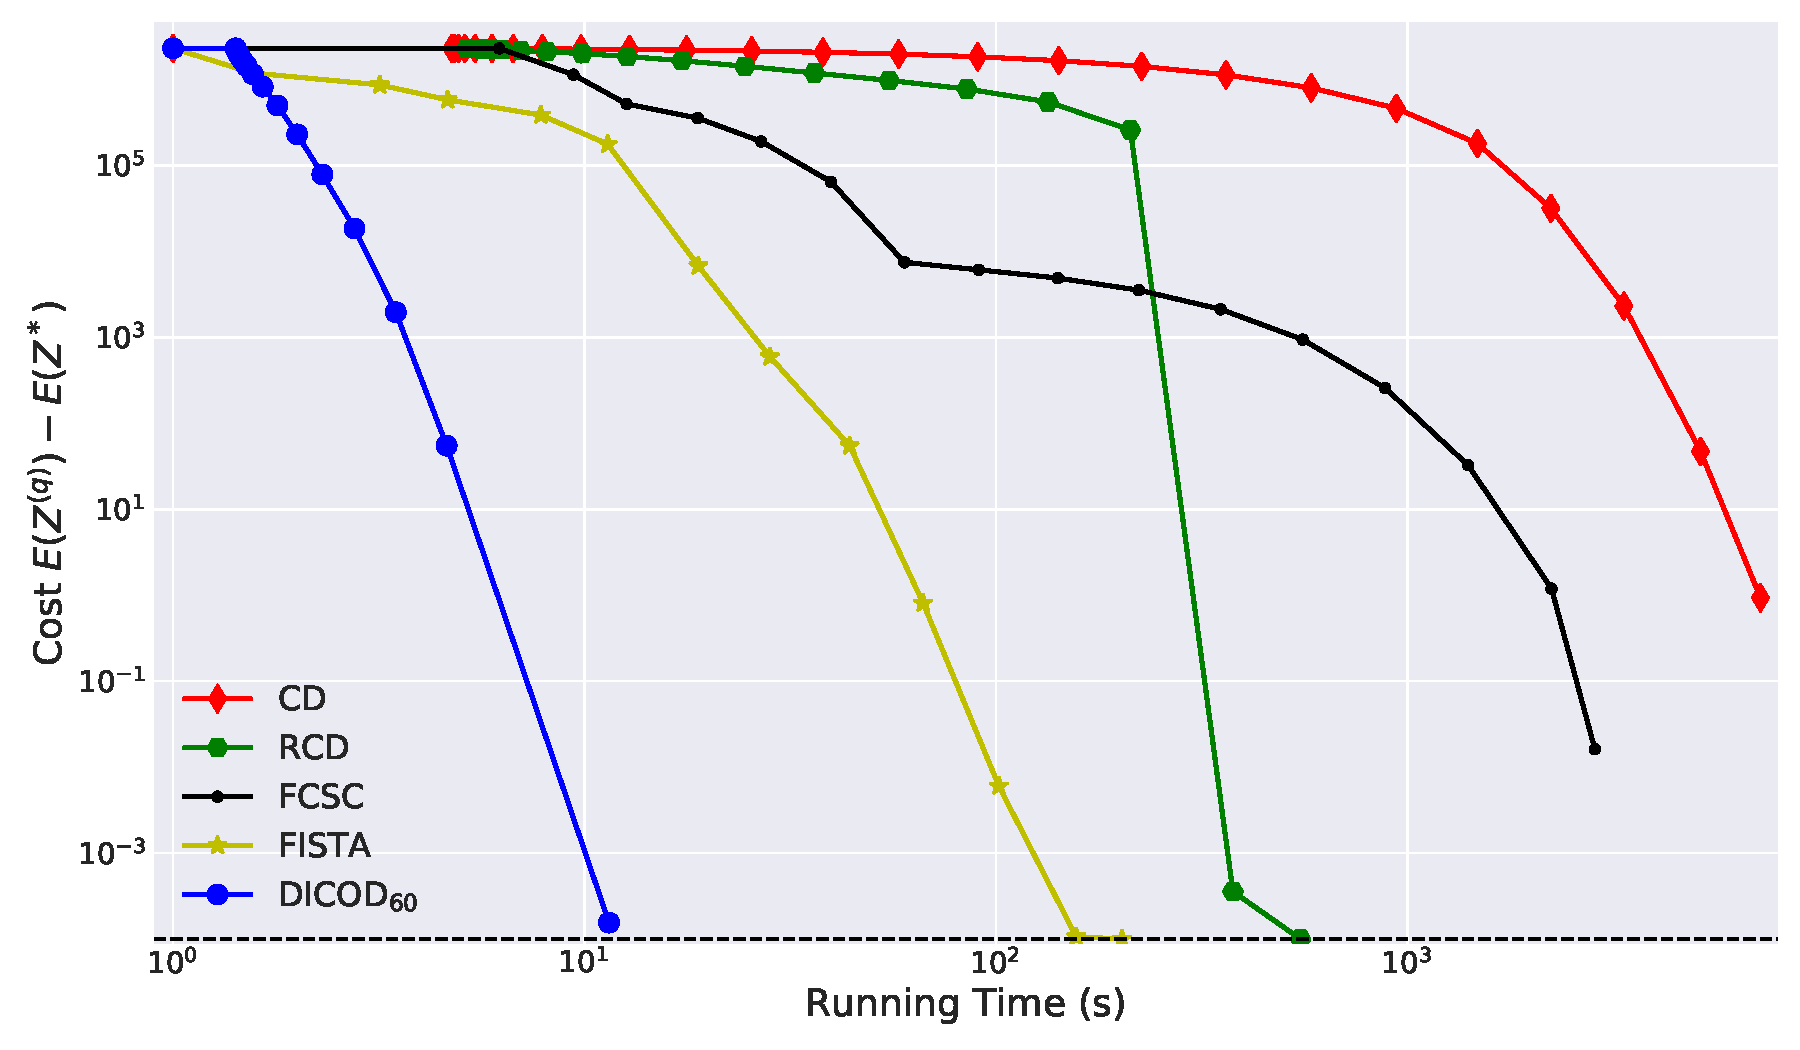
\includegraphics[width=.8\textwidth]{cost_min_seaborn_time}\\
    \large Cost as a function of the runtime\\
}{
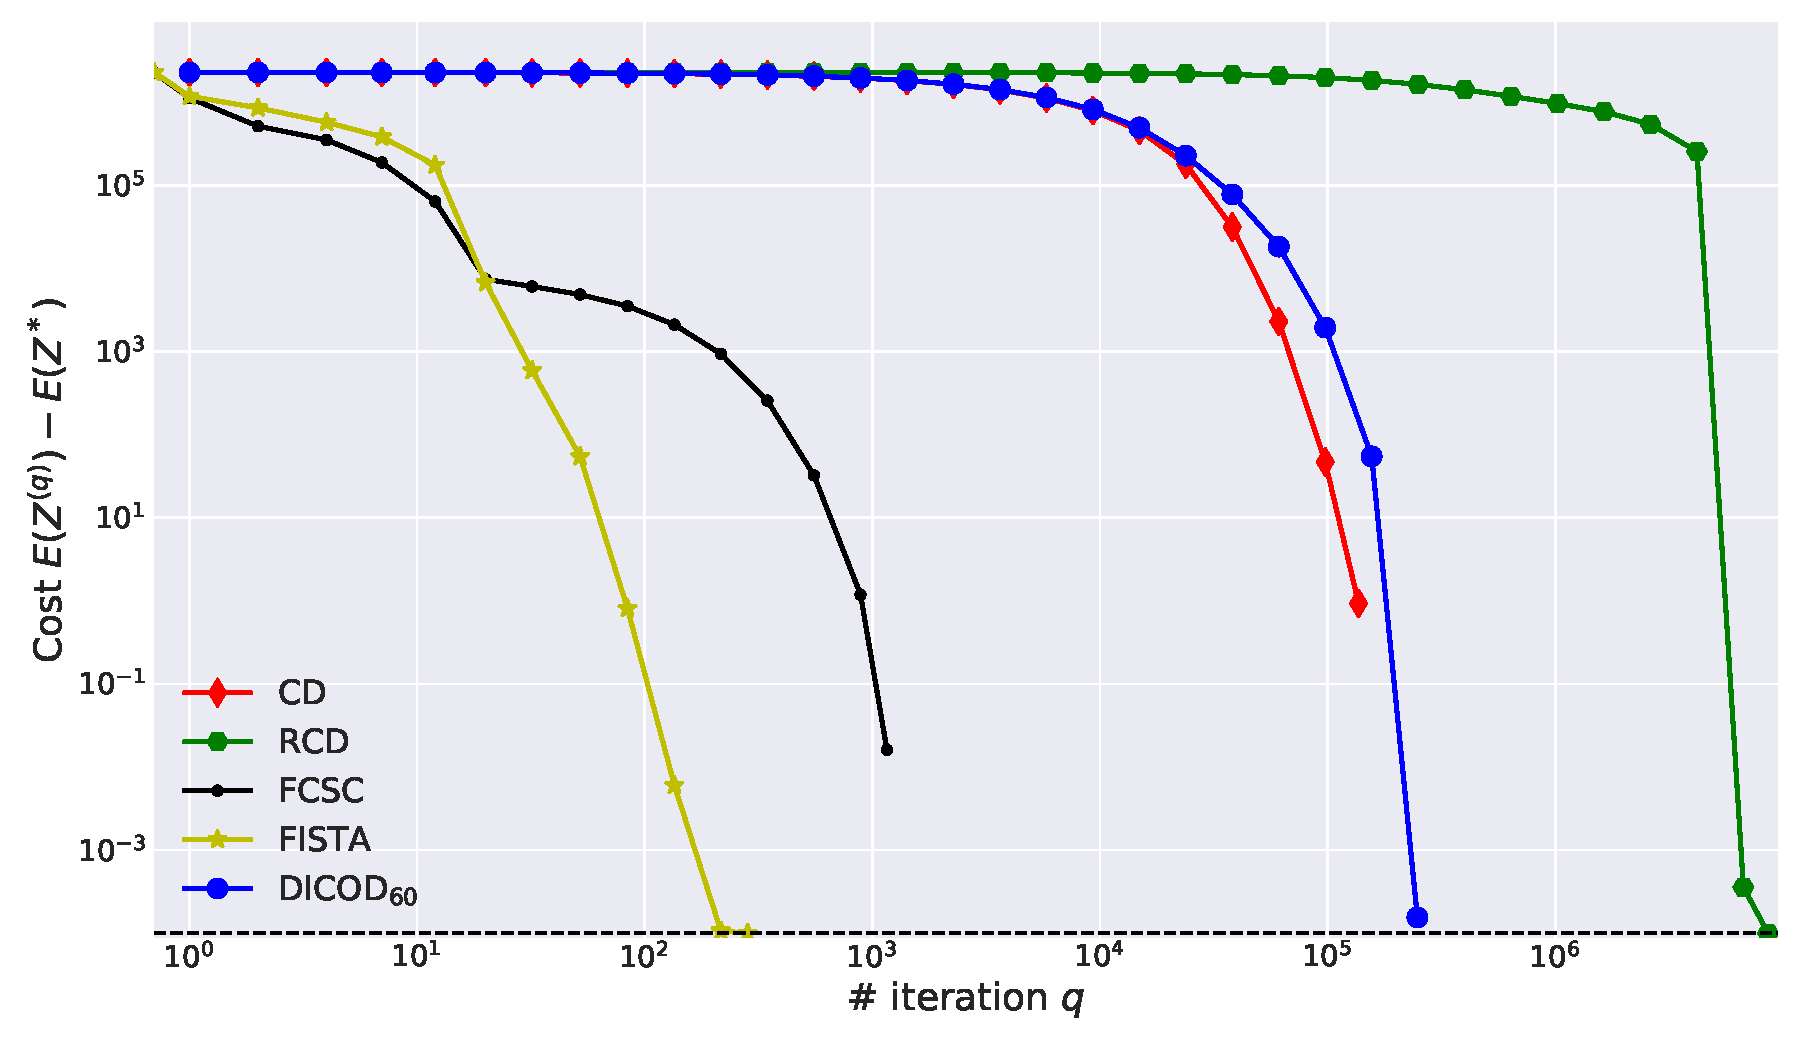
\includegraphics[width=.8\textwidth]{cost_min_seaborn_iter}\\
\large Cost as a function of the iterations\\
}
\end{frame}


\begin{frame}{Distributed Convolutional Dictionary Learning (DiCoDiLe-Z)}

\begin{columns}[c]
    \column{.5\textwidth}
    \includegraphics[width=.9\textwidth]{soft_lock_M49_support16_}
    \column{.5\textwidth}
    \begin{itemize}[<+->]\itemsep1em
        \item DICOD does not work for higher dimensional signals.
        \item Extension require to control interferences. 
        \item Use asynchronous mechanism: Soft-lock.
    \end{itemize}
\end{columns}

\end{frame}

\begin{frame}{Soft-Locks \mycite{Moreau2019}}

{
    \centering
    \inputTikZ{.7}{soft_lock}\\
}
\end{frame}


%\begin{frame}{Distributed Convolutional Dictionary Learning (DiCoDiLe-Z)}
%\vskip1em
%\begin{columns}[c]
%\column{.35\textwidth}
%\begin{itemize}\itemsep1em
%\only<1>{
%\item Update candidate $\omega_0$ is independent of other workers as
%\[
%\mathcal V(\omega_0) \subset \mathcal S_w
%\]
%}
%
%\only<2>{
%\item Update candidate $\omega_1$ impacts $\mathcal S_{w+1}$
%\[
%\mathcal V(\omega_1) \not\subset \mathcal S_w
%\]
%\item It is accepted only is no better update is possible in the "soft-locked" area.
%\item Need to notify $\mathcal S_{w+1}$.
%}
%\only<3>{
%\item Updates in $\omega_2$ need to notify worker $w$ to maintain consistent estimate in the border zone $\mathcal B_L(\mathcal S_w)$.
%
%\item Low communication: decentralized and below 1ko.
%}
%\end{itemize}
%\column{.65\textwidth}
%\inputTikZ{.75}{Sw_dicod.tex}
%\end{columns}
%\end{frame}


%---------------------------------------------------------------------------
\subsection{Complexity Analysis}
%---------------------------------------------------------------------------

\begin{frame}{Complexity Analysis}
	Two sources of acceleration:\\[1em]
	\begin{itemize}\itemsep1em
		\item Perform $M$ updates in parallel,
		\item Each update is computed on a segment of size $\frac{L}{M}$\\
		Iteration complexity of $\bO{K\frac{L}{M}}$ instead of $\bO{KL}$ 
	\end{itemize}
	\vskip1em
	Limitations:
	\begin{itemize}
	\item Interfering updates, with probability $\alpha^2 = \left(\frac{WM}{T}\right)^2$
	\[
		\mathbb E[Q_{dicod}] \smeq\underset{\alpha \to 0}{\gtrsim}
			M(1-2\alpha^2M^2 + \mathcal O(\alpha^4M^4))~.
	\]
	\item Cost of the update of $\beta$ in $\bO{KW}$  
\end{itemize}

\end{frame}

\begin{frame}{Numerical speed-up}

\centering
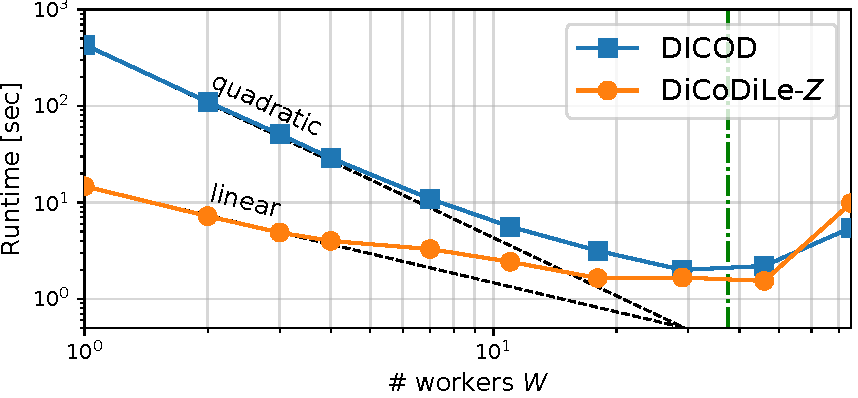
\includegraphics[width=\textwidth]{scaling_T150}
\\
\large Running time as a function fo the number of workers $W$.

\end{frame}



%%%%%%%%%%%%%%%%%%%%%%%%%%%%%%%%%%%%%%%%%%%%%%%%
%   Conclusion
%%%%%%%%%%%%%%%%%%%%%%%%%%%%%%%%%%%%%%%%%%%%%%%%

\begin{frame}{Contributions}

	\twocols{Contributions}{\vskip2em
	\begin{itemize}\itemsep.5em
		\item \underline{A novel algorithm DICOD:} distributed algorithm efficient to solve the
		CSC problem,
		\item \underline{Theoretical guarantees:} convergence to the optimal solution,
		\item \underline{Complexity analysis:} achieves a super-linear speedup
	\end{itemize}
	\vskip1.5em
	
	}{Future work}{\vskip2em
	\begin{itemize}\itemsep.5em
		\item Locally greedy coordinate descent
		\item 2D convolutions: extension of this algorithm to images,
		\item Local penalization: extension of this algorithm for localized penalties.
	\end{itemize}
	}
\end{frame}

\biblio{}
\end{document}